\chapter{Analýza pomocí metody 4ftMiner}
\label{ch:cleverminer}

Pomocí metody 4ftMiner, která je jednou z metod procedury GUHA jsem provedla analýzu shrinků produktu. Tato metoda je implemnetovaná v  knihovně \emph{Cleverminer} pro jazyk Python. Pracovala jsem pouze se vzorem dat jednoho měsíce a s kategorií produktů \emph{Velmi čerstvé} a \emph{Čerstvé}. Princip metod, které se používají v knihovně, a důležité pojmy týkající se GUHA procedur jsou popsány v sekci \ref*{sec:Teorie:Guha}. 

Zkoumaný dataset se záznamy shrinků produktů jsem rozšířila o další sledované sloupce, které dávají do srovnání hodnotu shrinku a objem tržeb. Vytvořila jsem takto sloupce: podíl shrinku na celkových tržbách prodejny, podíl shrinku na tržbách shrinkovaného produktu na prodejně, podíl shrinku a tržeb v kategorii úrovně 1.

Na základě zastoupení jednotlivých typů shrinků, kde prošlé a zkažené zboží zaujímá více než 64 \% shrinků, se následující analýzy zaměřují pouze na tento typ.

Metoda pracuje pouze s diskrétními hodnotami, proto bylo nutné kategorizovat sloupce s hodnotou shrinku, s množstvím shrinkovaných produktů a s jednotlivými podíly. Na obrázcích \ref*{obr:nb:hist} až \ref{obr:nb:hist5} jsou zobrazené četnosti záznamů v kategoriích.

\begin{figure}[h!]
    \centering
    \begin{minipage}[b]{.55\textwidth}
      \centering
      \captionsetup{justification=centering}

      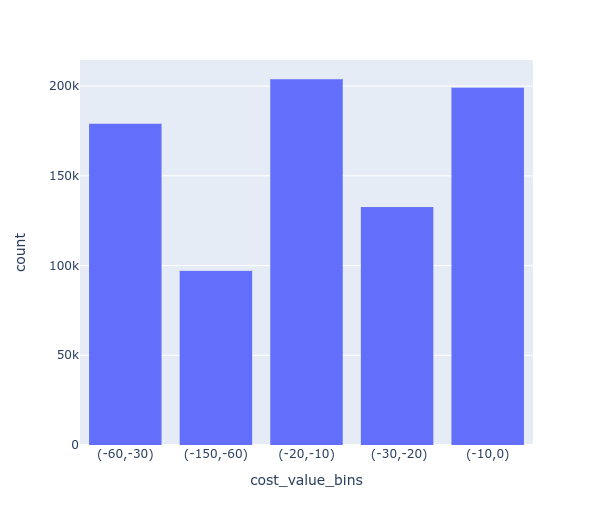
\includegraphics[width=\textwidth]{obrazky/grafy/histogram/newplot(2).png}
      \vspace*{-3em}
      \caption{Histogram pro hodnoty \\ velikosti shrinku v peněžních jednotkách.}
      \label{obr:nb:hist}
    \end{minipage}%
    \hspace*{-2em}
    \begin{minipage}[b]{.55\textwidth}
        \centering
        \captionsetup{justification=centering}
        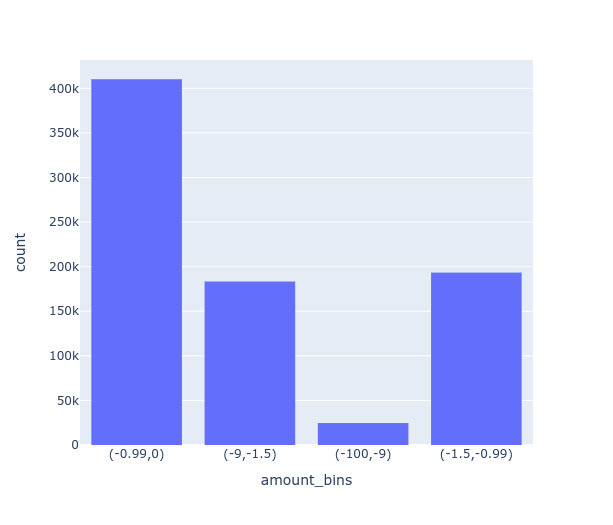
\includegraphics[width=\textwidth]{obrazky/grafy/histogram/newplot(1).png}
        \vspace*{-3em}
        \caption{Histogram pro hodnoty \\ objemu shrinku v kusech.}
        \label{obr:nb:hist2}
    \end{minipage}
\end{figure}
\vspace*{-2em}

\begin{figure}[h!]
    \centering
    \begin{minipage}[b]{.55\textwidth}
      \centering
      \captionsetup{justification=centering}

      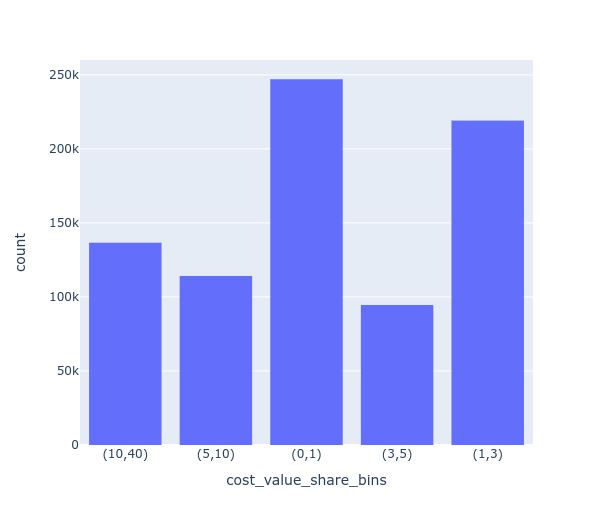
\includegraphics[width=\textwidth]{obrazky/grafy/histogram/newplot.png}
      \vspace*{-3em}
      \caption{Histogram podílu shrinku \\na tržbách shrinkovaného produktu.}
      \label{obr:nb:hist3}
    \end{minipage}%
    \hspace*{-2em}
    \begin{minipage}[b]{.55\textwidth}
        \centering
        \captionsetup{justification=centering}
  
        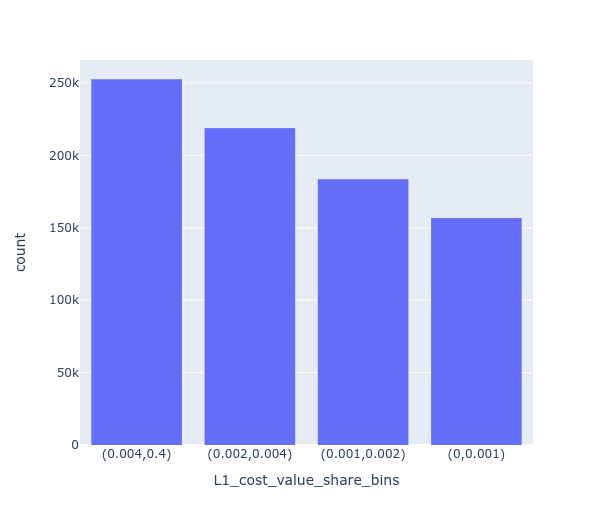
\includegraphics[width=\textwidth]{obrazky/grafy/histogram/newplot(3).png}
        \vspace*{-3em}
        \caption{Histogram podílu shrinku \\a tržeb v kategorii úrovně 1.}
        \label{obr:nb:hist4}
    \end{minipage}
\end{figure}

\begin{figure}[h!]
        \centering
        \captionsetup{justification=centering}
        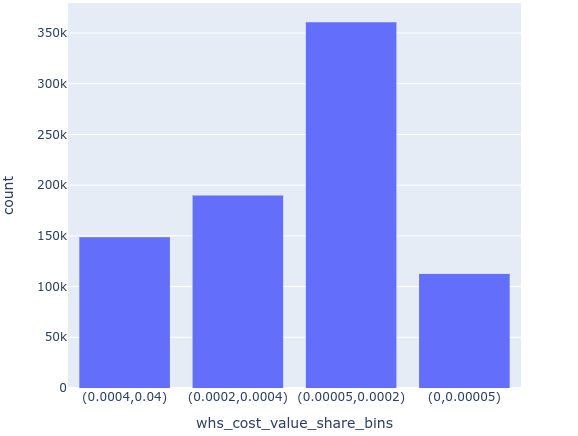
\includegraphics[width=0.55\textwidth]{obrazky/grafy/histogram/newplot(4).png}
        \caption{Histogram podílu shrinku \\na celkových tržbách prodejny.}
        \label{obr:nb:hist5}
\end{figure}

% TODO ukázky kategorizace TBD % TODO ukázky kategorizace TBD

\section{Hypotézy}

Data jsem analyzovala metodou \emph{4ftMiner}, které jsem nastavovala parametry podle zkoumané hypotézy. 

\subsubsection*{Hypotéza č. 1: Množství prošlého zboží je závislé na typu výprodeje a dni v týdnu}

V datech je zboží bez promoce zastoupeno $58{,}2$ \%, zboží v postpromočním výprodeji $23{,}2$, zboží v promoci $18{,}6$ procentem.

\subsubsection*{Hypotéza č. 2: Na některých lokalitách vyhazují často stejné produkty}

Nejčastější shrinkovanou kategorií jsou masné produkty (úroveň hierarchie 3). S větší než 60\% pravděpodobností tato kategorie byla zaznamenána u prodejen  v okresech: Cheb, Jindřichův Hradec, Kladno, Ústí nad Labem, Nymburk, Písek, Strakonice a Praha-východ. Pokud se vynechá v analýzách tato kategorie, pak se jedná o kategorii pečiva. Ta se s pracděpodobnostyí alespoň 60 \% týkala okresu Pardubice a Plzeň-město. Po vynechání je to kategorie zelenina, ovšem už jen s nejvyšší pravděpodobností pod 35 \%.

% |  4040 | 0.617 | +0.644 | **warehouse_type(HM) & region(Plzeň-město) => L3(SF CM BAKERY)**| --- |

\subsubsection*{Hypotéza č. 3: Na některých v některých lokalitách mají často zaznamenaný shrink}
\subsubsection*{Hypotéza č. 4: Některé produkty se vyhazují častěji než jiné, ale v malém množství.}

 Kategorie MEAT PRODUCTS (PROC. MEAT SERVICE)-( masné produkty, šunka, salámy, klobásy) byla zaznamenána téměř 300 tisíckrát, a v 90 procentech se jednalo o množství odpovídající do jednoho balení. 
%   Jedná o vážené pultové produkty - jde o
 Pokud se vyhazují čerstvé ryby (fresh fish), tak v 94 
\% záznamů je to množství do jednoho kusů. Tapas se vyhazují v 89 \% po jednom kusu (obvykle se jedná o sendviče a bagety)
Kategorie vejce se vyhazuje v 82 \% po jednom kusu balení
Kategorie pečiva se vyhazuje v 56 \% v počtu kusů do 10 ks v až 94 tis. záznamech.
Kategorie CORE FRUIT (hrušky a jablka) se vyhazuje 74 \% případech záznamů (14 000 záznamů) v množství do jednoho kusu - váhový přepočet.

\subsubsection*{Hypotéza č. 5: Některé vyhazované kategorie produktů jsou výrazně nákladnější.}

Pokud se vyhazují čerstvé ryby (fresh fish), tak v téměř 80 \% případech záznamů jsou ztracené náklady vyšší  - 60-150 balení.
Pokud se vyhazuje kategorie Red meat, tak z téměř 60 \% ve větším množství - 60-150 balení.
Kategorie CHILLED PRODUCT SERVICE, která obsahuje čerstvé chlebíčky, saláty a pochutiny na pultovém prodeji, se v 50 \% vyhazují v množství

\subsubsection*{Hypotéza č. 6: Shrink některých produktů je v porovnání s tržbami těchto produktů na stejné prodejně velký.}

Nejedná se o porovnání s celkovými tržbami prodejny, ale pouze o týdenní tržbu těch produktů, které měli zaznamenaný v daném týdnu shrink.
Tapas se mají share shrinku v 84 \% zaznamenaných případech mezi 10-40 \%.
 Cukrářské výrobky  mají share shrinku v 74 \% zaznamenaných případech mezi 10-40 \%.
 Banány mají share shrinku v 80 \% zaznamenaných případech do 1 \%.
 Více než 30 tis. záznamů je u Citrusů, Jablek a hrušek a v okolo 65 \% je share shrinku do 1 \%.

 Pokud mezi produkty, kterým byl zaznamenán dražší (30-60 Kč) shrink, jsou jogurty, tak jejich share shrinku na tržbách je mezi 10-40 \%, totéž se týká Tapas.
Pokud mezi produkty, kterým byl zaznamenán levný (do 10 Kč) shrink, je ovoce, tak jejich share shrinku na tržbách je do 1 \%, totéž se týká in kořenové zeleniny.

\subsubsection*{Hypotéza č. 7: Kategorie má vliv na zastoupení shrinku na celkových tržbách prodejny v dané kategorii úrovně 1.}

S pracděpodobností vyšší než 50 \% se toto tvrzení potvrdilo pouze u kategorie Bylinky z úrovně 4. Kdy (0.002,0.005).

\subsubsection*{Hypotéza č. 8: Den v týdnu nebo čtvrtina měsíce mají vliv na záznamy.}

Ve středu, čtvrtek a pátek v poslední čtvrtině měsíce je dvakrát více záznamů než v jiných dnech. Ostatní části měsíce jsou konzistentní.